\section{GAMYGDALA}
In the Gamygdala world, Agents have goals they want to achieve. Based on their beliefs, they assess whether or not they have achieved their goals, and for example what's the likelihood to achieve their goals. Based on these properties and based on the relation with other agents, the agent's emotion is calculated. \\ 

Each Agent has a separate Goal base which they update every evaluation cycle. Whenever an event happens, the impact on a particular goal has to be provided. New agent-specific values like the goal likelihood, change in likelihood, the overall utility of the goal (how useful is it to achieve the goal) are then recalculated. Finally, a new emotion is distilled from all these particular properties. \\

Because each goal is unique and interchangeable, the engine itself also keeps track of all goals. \\

\subsection{Porting}
In the process to porting the Gamygdala engine from Javascript to Java, we have implemented a number of design patterns to better structure the code. Since Gamygdala was originally developed as a gaming engine, we had to separate the core logic from other facilitator functions. The core logic is also separated into classes with a single-responsibility and coupling is avoided wherever possible. \\

During an analysis of the code, we found out that he five main classes of the engine are:
\begin{itemize}
	\item \textbf{Agent} The agent which interacts with the environment.
	\item \textbf{Goal} Goals which Agents want to achieve.
	\item \textbf{Belief} Beliefs which alter the Agent's view on the likelihood of achieving the goal.
	\item \textbf{Emotion} The Emotion which an Agent has after processing Beliefs (based on its Goals).
	\item \textbf{Relation} The Relation between two Agents.
\end{itemize}

To support our claim that we improved the code on the software engineering part, we made two UML-diagrams. The first diagram is made using our first version of the port, this was an almost exact copy of the original GAMYGDALA code. The second diagram is made using our re-factored code, it was not perfect but it was a big improvement over the original code. The UML-diagrams can be found on the next two pages.\\

\begin{figure}
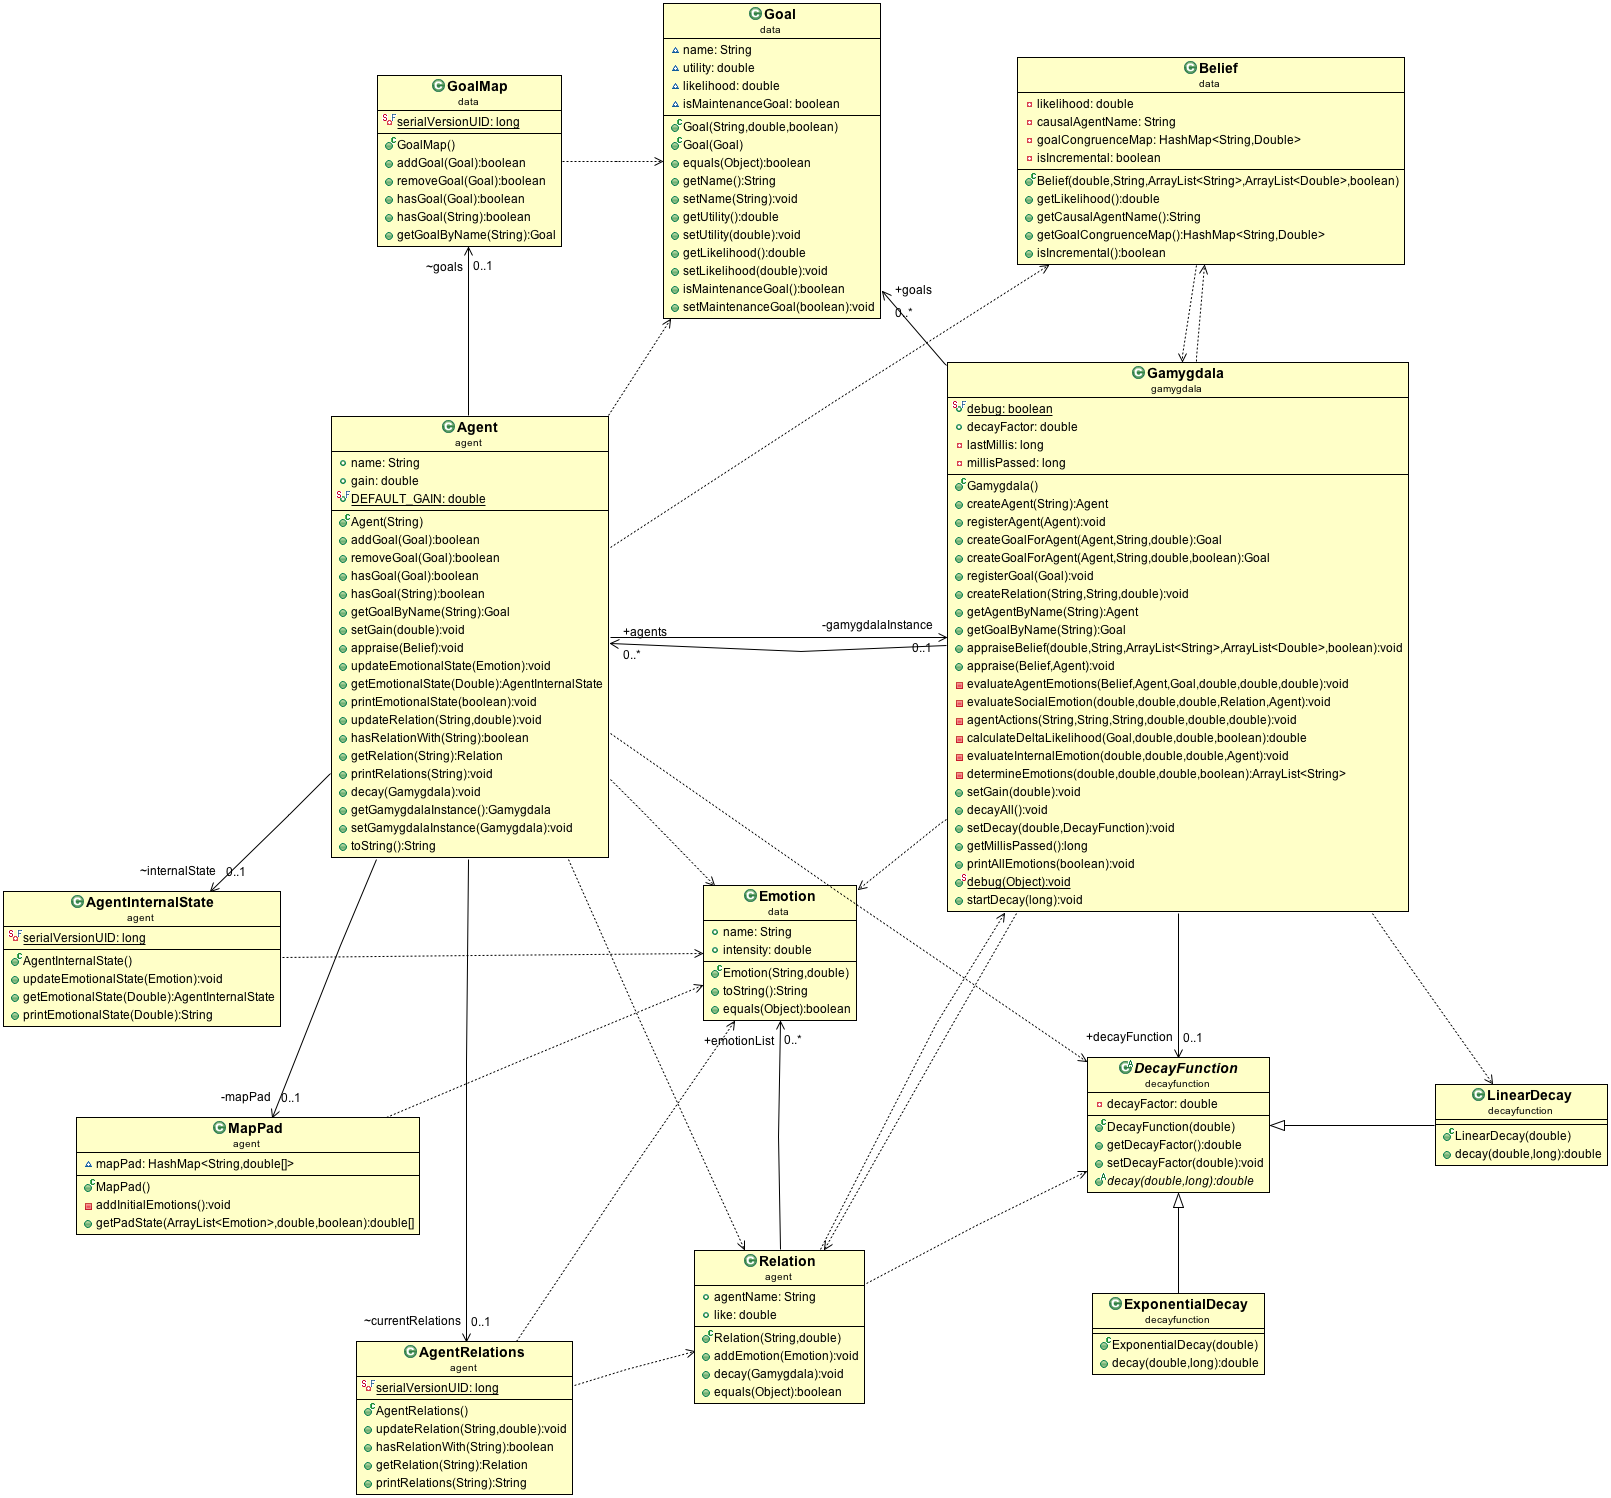
\includegraphics[width=\linewidth]{GAMYGDALA_UML_OLD}
\caption{The UML-diagram for the initial port.}
\end{figure}

\begin{figure}
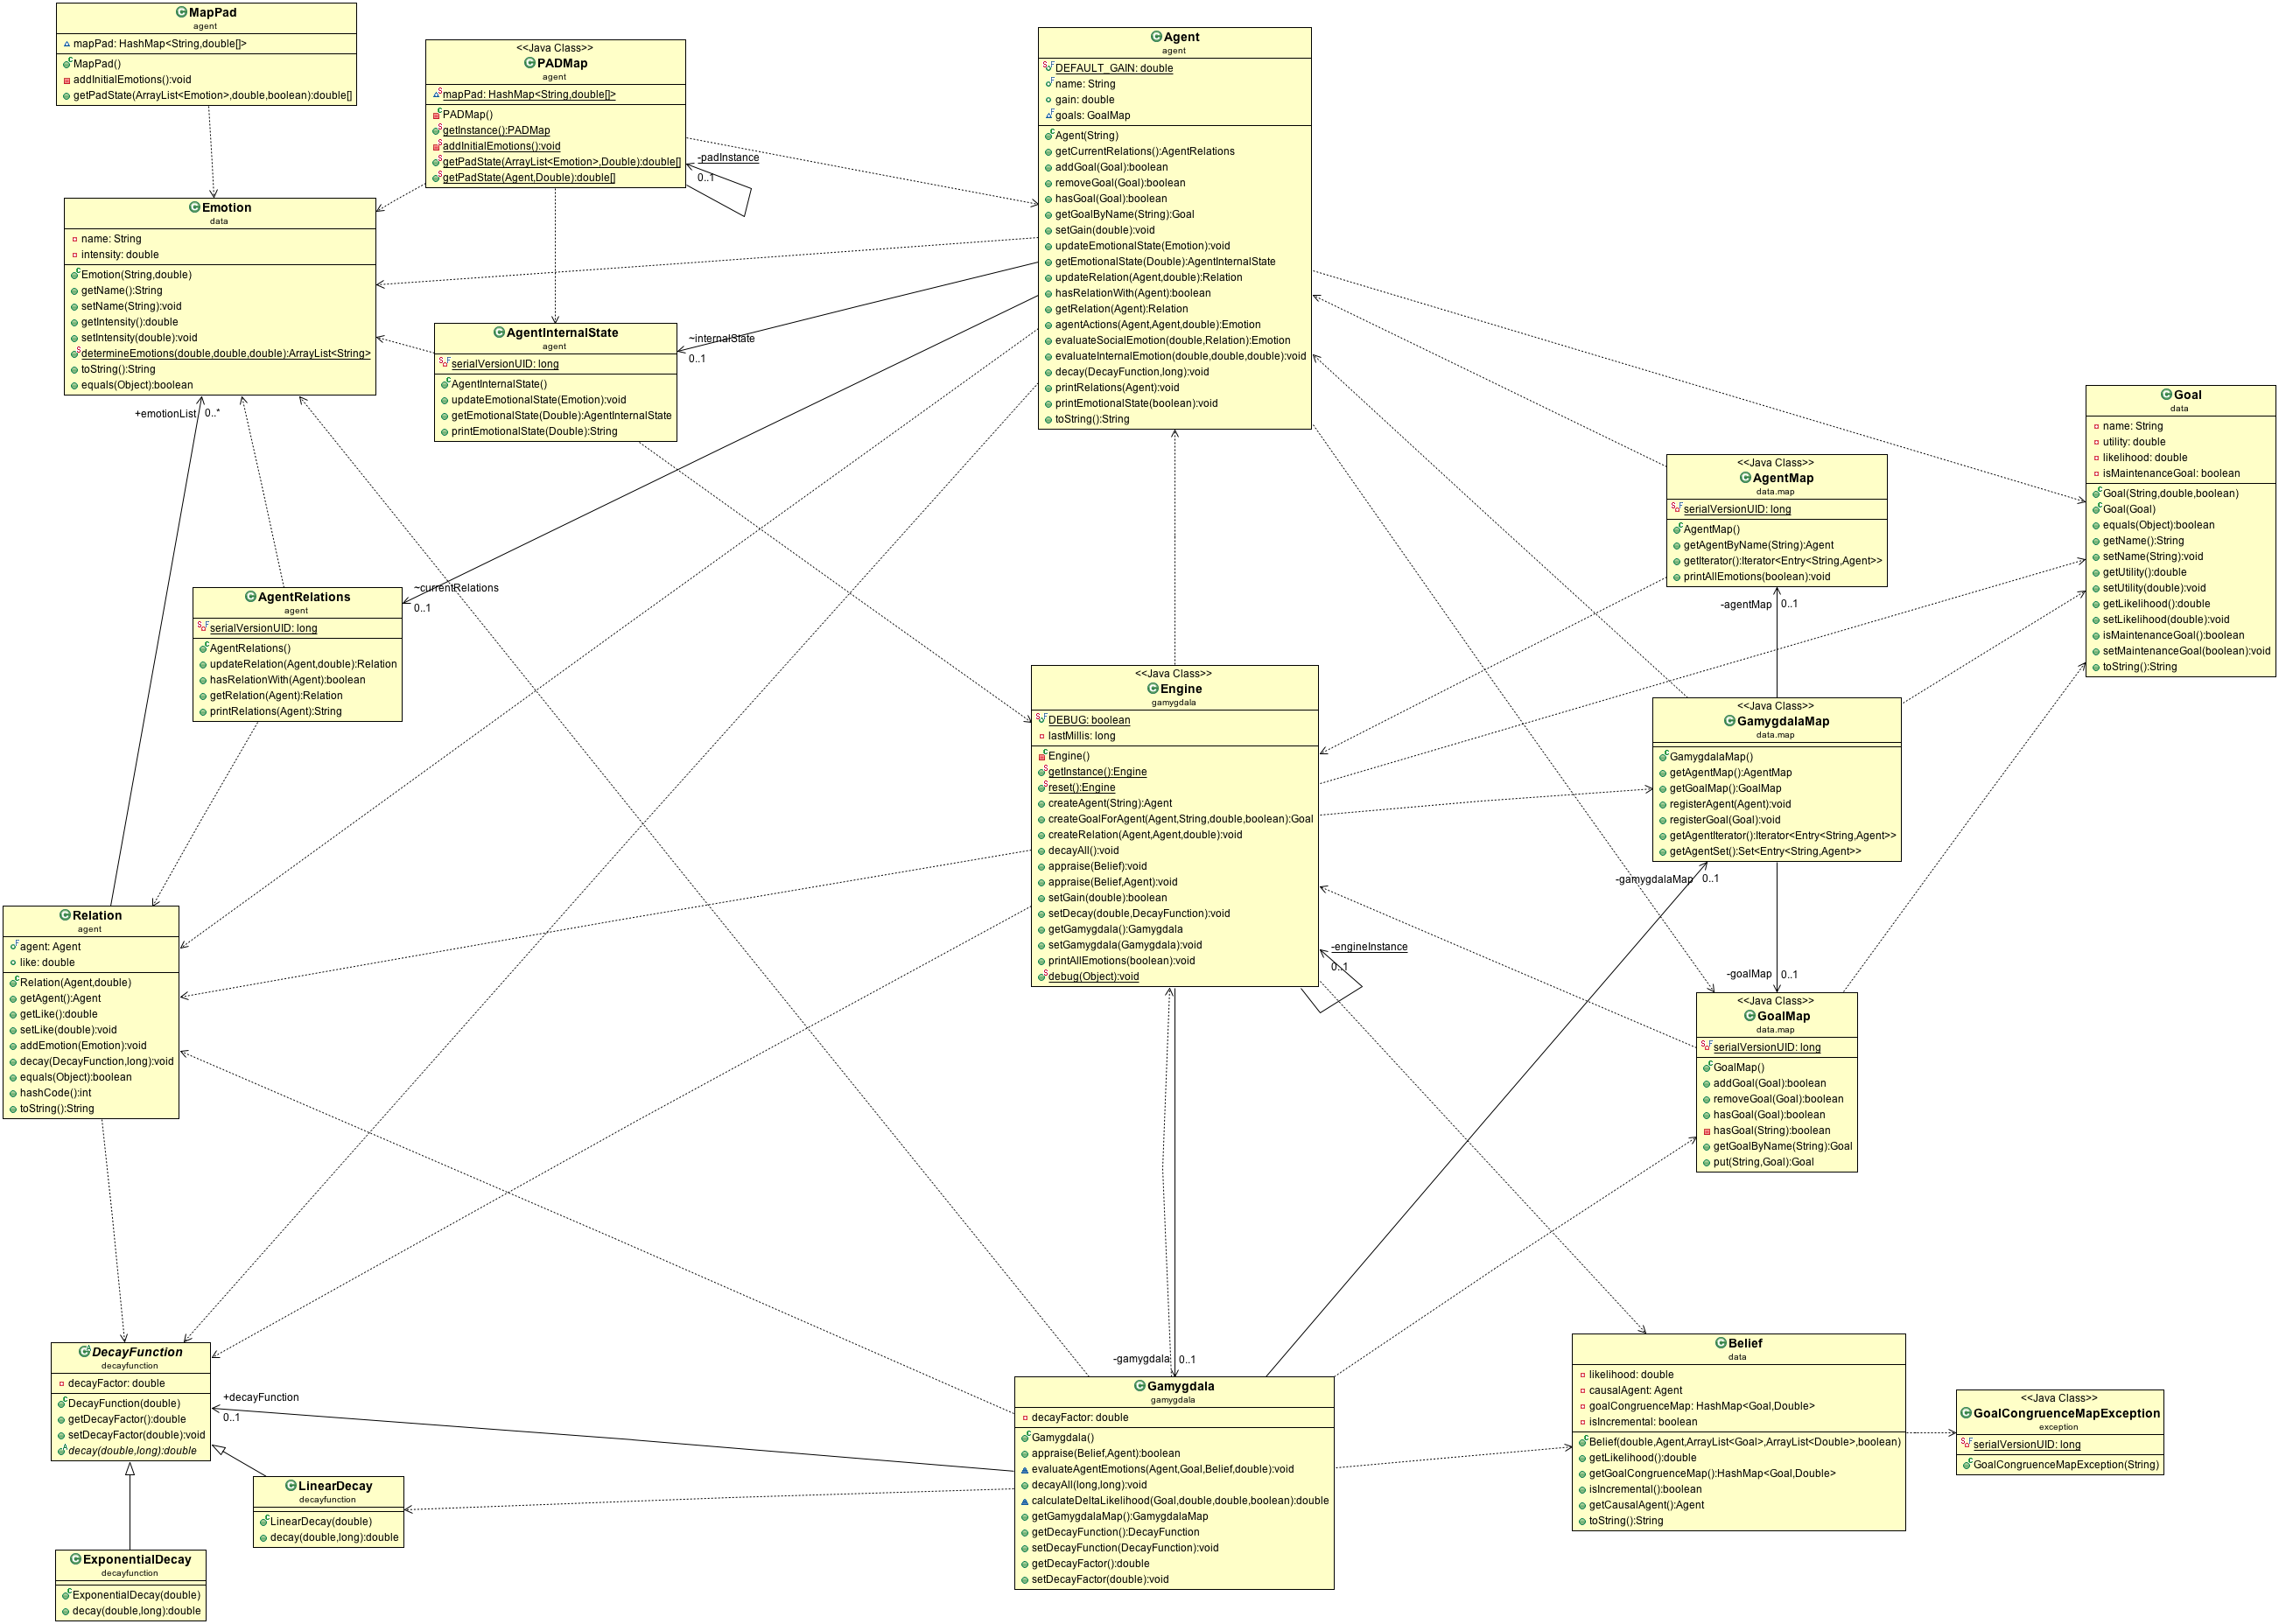
\includegraphics[width=\linewidth]{GAMYGDALA_UML_NEW}
\caption{The UML-diagram for the re-factored port.}
\end{figure}

\subsection{Test}

\subsection{Big re-factor}
After the initial port and re-factoring of GAMYGDALA, we came to the conclusion that the Java code was still not very pretty. It had long functions, big classes and still classes with multiple responsibilities. To counter these faults, we started a big re-factor of the code. First we divided some functions in smaller new functions with less responsibility. We distributed the smaller functions over different classes. These changes made the bigger classes smaller and gave them less responsibilities.  

\subsection{Benchmark}
When most of the 

\subsection{Design patterns}
Within the GAMYGDALA port there are several design patterns used. These patterns help to improve the code and make it easier to use and develop. In the following subsections, we will present to you the design patterns used within the code.

\subsubsection{Singleton pattern}
The singleton pattern is very usefull in cases where you want to have at most 1 object of a class. The Engine Class has the singleton pattern build in. This is because it is not useful to have two GAMYGDALA engines running beside each other. Emotions can be calculated for each agent, and relation too. So there is no need for a second engine. It could only confuse programmers if they had accidentally created two different GAMYGDALA engines and been working in them both.  
  
\subsubsection{Strategy pattern}
The strategy pattern is very usefull when you have something that needs to be calculated and it depends on certain conditions how it needs to be calculated. Because of this we used the strategy pattern to determine the kind of emotions. The emotion calculation is based on the likelihood. For certain values of the likelihood there is a different strategy to calculate the kind of emotion.